\documentclass[a4paper]{article}
\usepackage[T1]{fontenc}			% pacchetto per \chapter
\usepackage[italian]{babel}
\usepackage[italian]{isodate}  		% formato delle date in italiano
\usepackage{graphicx}				% gestione delle immagini
\usepackage{amsfonts}
\usepackage{booktabs}				% tabelle di qualità superiore
\usepackage{mathrsfs, amsmath}				% pacchetto matematica
\usepackage{mathtools}				% per sottolineare sotto le equazioni
\usepackage{stmaryrd} 				% per '\llbracket' e '\rrbracket'
\usepackage{amsthm}					% teoremi migliorati
\usepackage{enumitem}				% gestione delle liste
\usepackage{pifont}					% pacchetto con elenchi carini
\usepackage{enumitem}				% pacchetto per elenchi con lettere dell'alfabeto
\usepackage{cancel}					% per cancellare delle espressioni matematiche
\usepackage{listings}				% implementa codice di programmazione
\usepackage{mathalpha}
\usepackage{caption}


\usepackage[x11names]{xcolor}		% pacchetto colori RGB
% Link ipertestuali per l'indice
\usepackage{xcolor}
\usepackage[linkcolor=black, citecolor=blue, urlcolor=cyan]{hyperref}
\hypersetup{
	colorlinks=true
}

% Colour code style
\definecolor{codegreen}{rgb}{0,0.6,0}
\definecolor{codegray}{rgb}{0.5,0.5,0.5}
\definecolor{codepurple}{rgb}{0.58,0,0.82}
\definecolor{backcolour}{rgb}{0.95,0.95,0.92}

\lstdefinestyle{MATLAB}{
	backgroundcolor=\color{backcolour},   
	commentstyle=\color{codegreen},
	keywordstyle=\color{magenta},
	numberstyle=\tiny\color{codegray},
	stringstyle=\color{codepurple},
	basicstyle=\ttfamily\footnotesize,
	breakatwhitespace=false,         
	breaklines=true,                 
	captionpos=b,                    
	keepspaces=true,                 
	numbers=left,                    
	numbersep=5pt,                  
	showspaces=false,                
	showstringspaces=false,
	showtabs=false,                  
	tabsize=2
}
\lstset{style=MATLAB}

%\usepackage{showframe}				% visualizzazione bordi
%\usepackage{showkeys}				% visualizzazione etichetta

\newtheorem{theorem}{\textcolor{Red3}{\underline{Teorema}}}
\newtheorem{lemma}{Lemma}
\renewcommand{\qedsymbol}{QED}
\newcommand{\exec}[1]{\llbracket #1\:\rrbracket}
\newcommand{\dquotes}[1]{``#1''}
\newcommand{\longline}{\noindent\rule{\textwidth}{0.4pt}}

\begin{document}
	\author{Università degli Studi di Verona}
	\title{Soluzione - Simulazione di Elaborazione di segnali e immagini}
	\date{{\Large 15 Gennaio 2021}}
	\maketitle
	
	\section{Soluzione Esercizio}
	
	Prima di tutto si descrive analiticamente sia il segnale $X\left(\mu\right)$ che $Y\left(\mu\right)$. Il primo segnale è una box con ampiezza (altezza) $2$ e larga $4$ centrata nell'origine:
	\begin{equation*}
		\begin{array}{lllll}
			\text{Segnale nelle frequenze} & \longrightarrow & X\left(\mu\right) & = & 2 \cdot \Pi\left(\dfrac{\mu}{4}\right) \\
			\\
			\text{Segnale nel tempo} & \longrightarrow & x\left(t\right) & = & 2 \cdot 4 \mathrm{sinc}\left(4t\right) = 8\mathrm{sinc}\left(4t\right)
		\end{array}
	\end{equation*}
	Il secondo segnale è un triangolo con ampiezza $1$ e larga $2$ centrata nell'origine:
	\begin{equation*}
		\begin{array}{lllll}
			\text{Segnale nelle frequenze} & \longrightarrow & Y\left(\mu\right) & = & \Lambda\left(\dfrac{\mu}{1}\right) = \Lambda\left(\mu\right) \\
			\\
			\text{Segnale nel tempo} & \longrightarrow & y\left(t\right) & = & 1 \cdot \mathrm{sinc}^{2}\left(1t\right) = \mathrm{sinc}^{2}\left(t\right)
		\end{array}
	\end{equation*}
	Adesso è possibile eseguire le operazioni richieste dall'esercizio.\newpage
	
	\subsection*{\textcolor{Green4}{\underline{\textbf{\emph{Segnale $\boldsymbol{a\left(t\right)}$}}}}}
	
	Il segnale $a\left(t\right)$ si ottiene moltiplicando (\underline{nel tempo}) il segnale $x\left(t\right)$ con il segnale $\cos\left(2\pi5t\right)$. Per definizione, la moltiplicazione nel dominio del tempo corrisponde alla convoluzione nel dominio delle frequenze. Quindi, si sviluppa analiticamente l'operazione e infine si rappresenta graficamente:
	\begin{equation*}
		\begin{array}{lll}
			\text{Dominio del tempo} & \longrightarrow & a\left(t\right) = x\left(t\right) \cdot \cos\left(2\pi5t\right) \\
			\\
			\text{Dominio delle frequenze} & \longrightarrow & A\left(\mu\right) = X\left(\mu\right) * \dfrac{1}{2}\left(\delta\left(\mu+5\right) + \delta\left(\mu-5\right)\right)
		\end{array}
	\end{equation*}
	\noindent\fbox{%
		\parbox{\textwidth}{%
			\textbf{\emph{Richiamo della teoria}:} Il coseno $\cos$ è la somma di due impulsi shiftati. Infatti, data la sua forma generica:
			\begin{equation*}
				\cos\left(2 \pi f_{0} t\right)
			\end{equation*}
			La corrispettiva nel dominio delle frequenze:
			\begin{equation*}
				\dfrac{1}{2} \cdot \left(\delta\left(f+f_{0}\right) + \delta\left(f-f_{0}\right)\right)
			\end{equation*}
			Dove $f_{0}$ rappresenta la posizione dell'impulso.\newline
			
			\noindent
			Analogamente, il seno $\sin$ è la differenza di due impulsi shiftati. Infatti, data la sua forma generica:
			\begin{equation*}
				\sin\left(2 \pi f_{0} t\right)
			\end{equation*}
			La corrispettiva nel dominio delle frequenze:
			\begin{equation*}
				\dfrac{1}{2}j \cdot \left(\delta\left(f+f_{0}\right) - \delta\left(f-f_{0}\right)\right)
			\end{equation*}
			Dove $f_{0}$ rappresenta la posizione dell'impulso e la $j$ è la parte immaginaria.
		}%
	}\newpage
	
	\noindent
	Si sviluppa la convoluzione\footnote{La formula della convoluzione è: $f_{1} * f_{2}\left(t\right) = \displaystyle\int_{-\infty}^{\infty} f_{1}\left(\tau\right) f_{2}\left(t-\tau\right) \: \mathrm{d}\tau$} sfruttando la proprietà di setacciamento\footnote{Il setacciamento può essere applicato nel caso in cui l'impulso sia coinvolto nella convoluzione e dunque $\displaystyle\int_{-\infty}^{\infty}f\left(x\right) \delta\left(x-x_{0}\right)\: \mathrm{d}t = f\left(x_{0}\right)$} per rimuovere elegantemente l'integrale:
	\begin{equation*}
		\begin{array}{lll}
			A\left(\mu\right) & = & X\left(\mu\right) * \dfrac{1}{2}\left(\delta\left(\mu+5\right) + \delta\left(\mu-5\right)\right) \\
			\\
			& = & \displaystyle\int_{-\infty}^{\infty} X\left(\tau\right) \cdot \dfrac{1}{2}\left(\delta\left(\mu+5-\tau\right) + \delta\left(\mu-5-\tau\right)\right) \: \mathrm{d}\tau \\
			\\
			& \downarrow & \text{Porto fuori } \frac{1}{2} \\
			\\
			& = & \dfrac{1}{2} \cdot \displaystyle\int_{-\infty}^{\infty} X\left(\tau\right) \cdot \left(\delta\left(\mu+5-\tau\right) + \delta\left(\mu-5-\tau\right)\right) \: \mathrm{d}\tau \\
			\\
			& \downarrow & \text{Moltiplico i due impulsi per il segnale } X\left(\tau\right) \\
			\\
			& = & \dfrac{1}{2} \cdot \displaystyle\int_{-\infty}^{\infty} \left[X\left(\tau\right) \cdot \delta\left(\mu+5-\tau\right)\right] + \left[X\left(\mu\right) \cdot \delta\left(\mu-5-\tau\right)\right] \: \mathrm{d}\tau \\
			\\
			& \downarrow & \text{Proprietà della somma degli integrali e divido i termini} \\
			\\
			& = & \dfrac{1}{2} \left( \displaystyle\int_{-\infty}^{\infty}X\left(\tau\right) \cdot \delta\left(\mu+5-\tau\right) \: \mathrm{d}\tau + \displaystyle\int_{-\infty}^{\infty}X\left(\tau\right) \cdot \delta\left(\mu-5-\tau\right) \: \mathrm{d}\tau \right) \\
			\\
			& \downarrow & \text{Proprietà di setacciamento} \\
			\\
			& = & \dfrac{1}{2} \cdot \left(X\left(\mu+5\right) + X\left(\mu-5\right)\right) \\
			\\
			& \downarrow & \text{Riunisco i termini per comodità} \\
			\\
			& = & \dfrac{1}{2}X\left(\mu+5\right) + \dfrac{1}{2}X\left(\mu-5\right) \\
			\\
			& \downarrow & \text{Sostituisco il segnale } X\left(\mu\right) \text{ con quello calcolato: } 2\cdot\Pi\left(\frac{\mu}{4}\right) \\
			\\
			& = & \dfrac{1}{2} \cdot 2 \Pi\left(\dfrac{\mu + 5}{4}\right) + \dfrac{1}{2} \cdot 2 \Pi\left(\dfrac{\mu - 5}{4}\right) \\
			\\
			& \downarrow & \text{Eseguo i calcoli} \\
			\\
			& = & \Pi\left(\dfrac{\mu + 5}{4}\right) + \Pi\left(\dfrac{\mu - 5}{4}\right)
		\end{array}
	\end{equation*}\newpage

	\noindent
	Il segnale è nel dominio delle frequenze. Si traduce anche nel dominio del tempo. Sapendo che:
	\begin{equation*}
		\Pi\left(\dfrac{\mu}{4}\right) \longrightarrow 4\mathrm{sinc}\left(4t\right)
	\end{equation*}
	Lo shift nel tempo è possibile scriverlo utilizzando l'esponenziale:
	\begin{equation*}
		\Pi\left(\dfrac{\mu + 5}{4}\right) + \Pi\left(\dfrac{\mu - 5}{4}\right) \longrightarrow 4\mathrm{sinc}\left(4t\right) e^{j 2 \pi 5 t} + 4\mathrm{sinc}\left(4t\right) e^{-j 2 \pi 5 t}
	\end{equation*}
	Raggruppando i termini comuni:
	\begin{equation*}
		4\mathrm{sinc}\left(4t\right) + 4\mathrm{sinc}\left(4t\right) \longrightarrow 4\mathrm{sinc}\left(4t\right)\left(e^{j 2 \pi 5 t} + e^{-j 2 \pi 5 t}\right)
	\end{equation*}
	Grazie alla formula di Eulero del coseno, è noto che esso è possibile riscriverlo:
	\begin{equation*}
		\cos\left(x\right) = \dfrac{e^{ix} + e^{-ix}}{2}
	\end{equation*}
	La forma che si ha è simile, ma manca la divisione. Tuttavia, è possibile scrivere il coseno, inserendo una moltiplicazione per due così da fare una manipolazione algebrica. Quindi:
	\begin{equation*}
		4\mathrm{sinc}\left(4t\right)\left(e^{j 2 \pi 5 t} + e^{-j 2 \pi 5 t}\right) \xlongrightarrow{\text{Eulero}} 4\mathrm{sinc}\left(4t\right) \cdot 2 \cos\left(2 \pi 5 t\right)
	\end{equation*}
	Quindi, nel dominio del tempo, il segnale $a\left(t\right)$ è il seguente:
	\begin{equation*}
		a\left(t\right) = 4\mathrm{sinc}\left(4t\right) \cdot 2 \cos\left(2 \pi 5 t\right)
	\end{equation*}
	\begin{figure}[!htp]
		\centering
		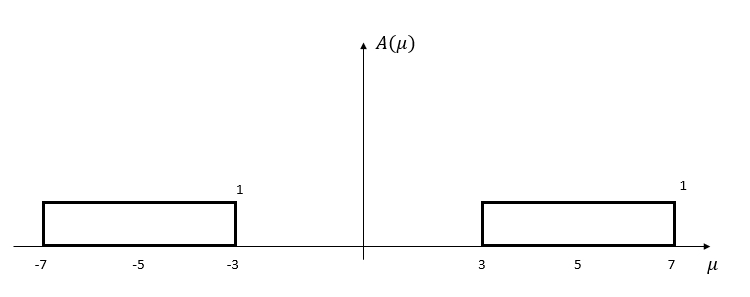
\includegraphics[width=\textwidth]{img/fig_1.png}
		\caption*{Rappresentazione grafica del segnale $A\left(\mu\right)$ nel dominio delle frequenze.}
	\end{figure}\newpage
	
	\subsection*{\textcolor{Green4}{\underline{\textbf{\emph{Segnale $\boldsymbol{b\left(t\right)}$}}}}}
		
	Come per il segnale $a\left(t\right)$, anche il segnale $b\left(t\right)$ si ottiene tramite una convoluzione nel dominio delle frequenze poiché si ha una moltiplicazione nel dominio del tempo. In questo caso, si saltano alcune spiegazioni, i passaggi specifici sono identici al segnale precedente.
	\begin{equation*}
		\begin{array}{lll}
			\text{Dominio del tempo} & \longrightarrow & b\left(t\right) = y\left(t\right) \cdot \cos\left(2\pi4t\right) \\
			\\
			\text{Dominio delle frequenze} & \longrightarrow & B\left(\mu\right) = Y\left(\mu\right) * \dfrac{1}{2}\left(\delta\left(\mu+4\right) + \delta\left(\mu-4\right)\right)
		\end{array}
	\end{equation*}
	\noindent
	Si sviluppa la convoluzione sfruttando la proprietà di setacciamento per rimuovere elegantemente l'integrale:
	\begin{equation*}
		\begin{array}{lll}
			B\left(\mu\right) & = & Y\left(\mu\right) * \dfrac{1}{2}\left(\delta\left(\mu+4\right) + \delta\left(\mu-4\right)\right) \\
			\\
			& = & \displaystyle\int_{-\infty}^{\infty} Y\left(\tau\right) \cdot \dfrac{1}{2}\left(\delta\left(\mu+4-\tau\right) + \delta\left(\mu-4-\tau\right)\right) \: \mathrm{d}\tau \\
			\\
			& = & \dfrac{1}{2} \cdot \displaystyle\int_{-\infty}^{\infty} Y\left(\tau\right) \cdot \left(\delta\left(\mu+4-\tau\right) + \delta\left(\mu-4-\tau\right)\right) \: \mathrm{d}\tau \\
			\\
			& = & \dfrac{1}{2} \cdot \displaystyle\int_{-\infty}^{\infty} \left[Y\left(\tau\right) \cdot \delta\left(\mu+4-\tau\right)\right] + \left[Y\left(\mu\right) \cdot \delta\left(\mu-4-\tau\right)\right] \: \mathrm{d}\tau \\
			\\
			& = & \dfrac{1}{2} \left( \displaystyle\int_{-\infty}^{\infty}Y\left(\tau\right) \cdot \delta\left(\mu+4-\tau\right) \: \mathrm{d}\tau + \displaystyle\int_{-\infty}^{\infty}Y\left(\tau\right) \cdot \delta\left(\mu-4-\tau\right) \: \mathrm{d}\tau \right) \\
			\\
			& = & \dfrac{1}{2} \cdot \left(Y\left(\mu+4\right) + Y\left(\mu-4\right)\right) \\
			\\
			& = & \dfrac{1}{2}Y\left(\mu+4\right) + \dfrac{1}{2}Y\left(\mu-4\right) \\
			\\
			& = & \dfrac{1}{2} \cdot \Lambda\left(\mu + 4\right) + \dfrac{1}{2} \cdot \Lambda\left(\mu - 4\right)
		\end{array}
	\end{equation*}
	Si scrive il segnale nel dominio del tempo ricordando che il triangolo è un $\mathrm{sinc}^{2}$:
	\begin{equation*}
		b\left(t\right) = \dfrac{1}{2} \cdot \mathrm{sinc}^{2}\left(t\right) e^{j 2 \pi 4 t} + \dfrac{1}{2} \cdot \mathrm{sinc}^{2}\left(t\right) e^{-j 2 \pi 4 t}
	\end{equation*}
	Come per il segnale precedente, si raccoglie l'esponenziale e si applica Eulero:
	\begin{equation*}
		\dfrac{1}{2} \mathrm{sinc}^{2}\left(t\right) \left(e^{j 2 \pi 4 t} + e^{-j 2 \pi 4 t}\right) \xlongrightarrow{\text{Eulero}} \dfrac{1}{2} \mathrm{sinc}^{2}\left(t\right) \cdot 2 \cos \left(j 2 \pi 4 t\right)
	\end{equation*}
	Quindi il segnale è:
	\begin{equation*}
		b\left(t\right) = \dfrac{1}{2} \mathrm{sinc}^{2}\left(t\right) \cdot 2\cos\left(2 \pi 4 t\right)
	\end{equation*}\newpage

	\begin{figure}[!htp]
		\centering
		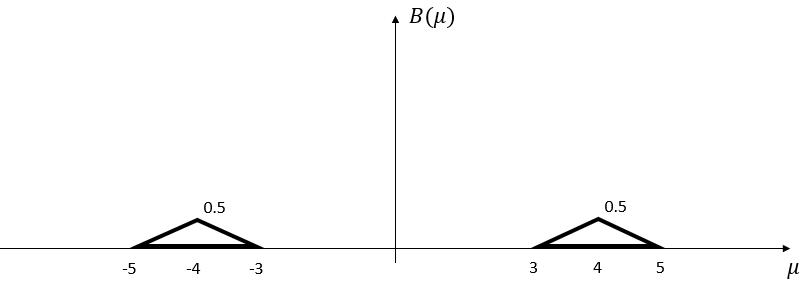
\includegraphics[width=\textwidth]{img/fig_2.png}
		\caption*{Rappresentazione grafica del segnale $B\left(\mu\right)$ nel dominio delle frequenze.}
	\end{figure}\newpage
	
	\subsection*{\textcolor{Green4}{\underline{\textbf{\emph{Segnale $\boldsymbol{c\left(t\right)}$}}}}}
	
	Campionare un segnale significa moltiplicarlo per un treno di impulsi. Quest'ultimi sono posti ad una distanza specifica. In questo esercizio la frequenza è pari a $15$ Hz, dunque ogni $15$ il segnale viene ripetuto. Le operazioni sono banali e prevedono una moltiplicazione del segnale per il treno di impulsi nel dominio del tempo e una convoluzione del segnale con un treno di impulsi.\newline
	
	\noindent
	Il segnale nel dominio del tempo è dunque la sommatoria degli impulsi per il segnale:
	\begin{equation*}
		c\left(t\right) = a\left(t\right) \cdot \displaystyle\sum_{n} \delta\left(\dfrac{t-n}{15}\right)
	\end{equation*}
	Nel dominio delle frequenze è necessario fare la convoluzione, quindi:
	\begin{equation*}
		\begin{array}{lll}
			C\left(\mu\right) & = & A\left(\mu\right) * 15\displaystyle\sum_{n} \delta\left(\mu - 15n\right) \\
			\\
			& = & \displaystyle\int_{-\infty}^{\infty} A\left(\tau\right) \cdot 15\displaystyle\sum_{n} \delta\left(\mu - 15n - \tau\right) \: \mathrm{d}\tau \\
			\\
			& \downarrow & \text{Porto fuori il } 15 \\
			\\
			& = & 15 \cdot \displaystyle\int_{-\infty}^{\infty} A\left(\tau\right) \cdot \displaystyle\sum_{n} \delta\left(\mu - 15n - \tau\right) \: \mathrm{d}\tau \\
			\\
			& \downarrow & \text{Proprietà di setacciamento} \\
			\\
			& = & 15 \cdot \displaystyle\sum A\left(\mu - 15n\right)
		\end{array}
	\end{equation*}
	\begin{figure}[!htp]
		\centering
		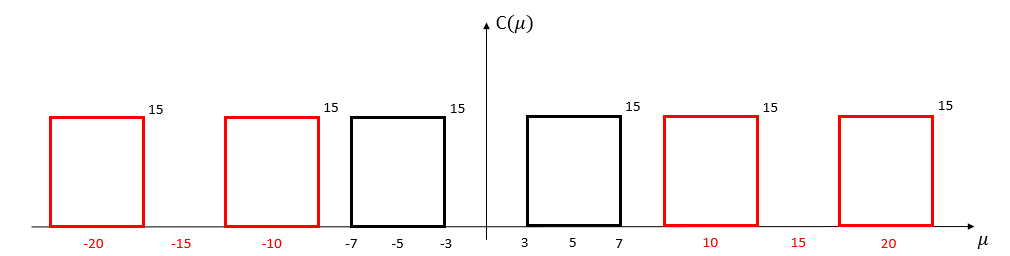
\includegraphics[width=\textwidth]{img/fig_3.png}
		\caption*{Rappresentazione grafica del segnale $C\left(\mu\right)$ nel dominio delle frequenze.}
	\end{figure}\newpage

	\subsection*{\textcolor{Green4}{\underline{\textbf{\emph{Segnale $\boldsymbol{d\left(t\right)}$}}}}}
	
	Come per il segnale precedente, anche in questo caso si applica il campionamento. La frequenza è identica e ancora una volta si esegue la moltiplicazione nel dominio del tempo e la convoluzione nel dominio delle frequenze.\newline
	
	\noindent
	Il segnale nel dominio del tempo è dunque la sommatoria degli impulsi per il segnale:
	\begin{equation*}
		d\left(t\right) = b\left(t\right) \cdot \displaystyle\sum_{n} \delta\left(\dfrac{t-n}{15}\right)
	\end{equation*}
	Nel dominio delle frequenze è necessario fare la convoluzione, quindi:
	\begin{equation*}
		\begin{array}{lll}
			D\left(\mu\right) & = & B\left(\mu\right) * 15\displaystyle\sum_{n} \delta\left(\mu - 15n\right) \\
			\\
			& = & \displaystyle\int_{-\infty}^{\infty} B\left(\tau\right) \cdot 15\displaystyle\sum_{n} \delta\left(\mu - 15n - \tau\right) \: \mathrm{d}\tau \\
			\\
			& \downarrow & \text{Porto fuori il } 15 \\
			\\
			& = & 15 \cdot \displaystyle\int_{-\infty}^{\infty} B\left(\tau\right) \cdot \displaystyle\sum_{n} \delta\left(\mu - 15n - \tau\right) \: \mathrm{d}\tau \\
			\\
			& \downarrow & \text{Proprietà di setacciamento} \\
			\\
			& = & 15 \cdot \displaystyle\sum B\left(\mu - 15n\right)
		\end{array}
	\end{equation*}
	\begin{figure}[!htp]
		\centering
		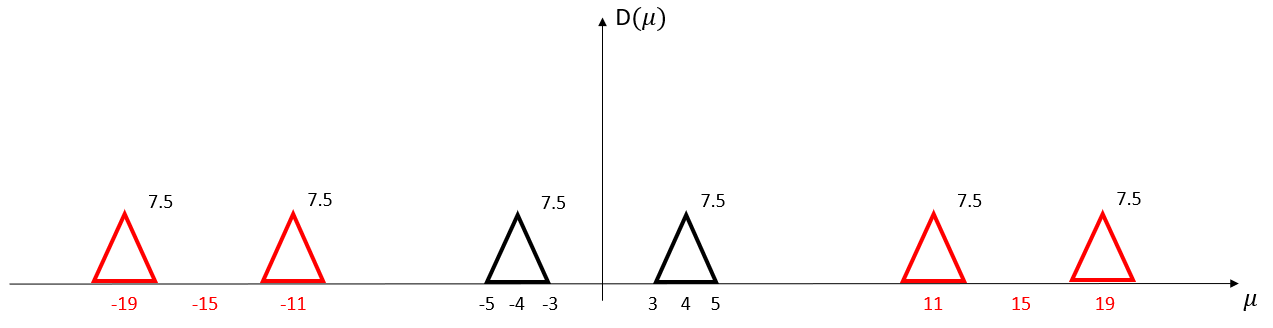
\includegraphics[width=\textwidth]{img/fig_4.png}
		\caption*{Rappresentazione grafica del segnale $D\left(\mu\right)$ nel dominio delle frequenze.}
	\end{figure}\newpage

	\subsection*{\textcolor{Green4}{\underline{\textbf{\emph{Segnale $\boldsymbol{e\left(t\right)}$}}}}}
	
	Il segnale finale si ottiene tramite la somma dei segnali. La somma è banale poiché analiticamente è immediato e graficamente basta rappresentare una somma dei valori dei segnali:
	\begin{equation*}
		\begin{array}{lll}
			\text{Dominio nel tempo} 		& \longrightarrow & e\left(t\right) = c\left(t\right) + d\left(t\right) \\
			\\
			\text{Dominio nelle frequenze} 	& \longrightarrow & E\left(\mu\right) = C\left(\mu\right) + D\left(\mu\right)
		\end{array}
	\end{equation*}
	\begin{figure}[!htp]
		\centering
		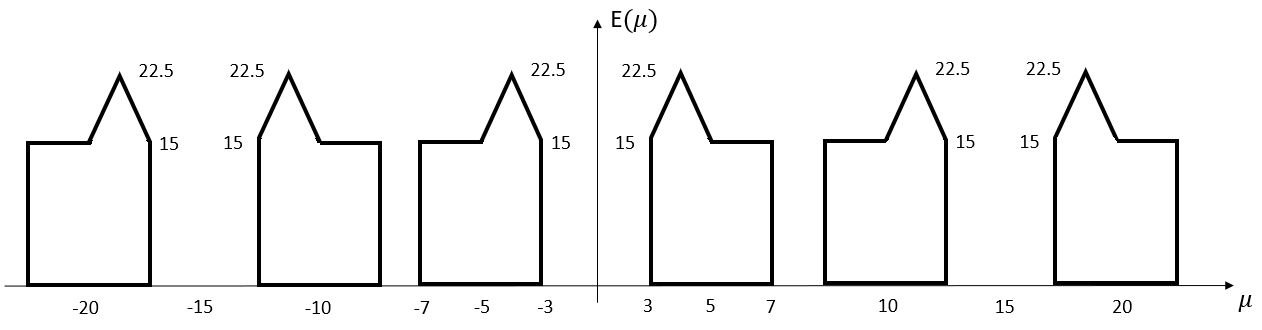
\includegraphics[width=\textwidth]{img/fig_5.png}
		\caption*{Rappresentazione grafica del segnale $E\left(\mu\right)$ nel dominio delle frequenze.}
	\end{figure}\newpage

	\section{Soluzione Esercizio}
	
	Dato il segnale nel dominio del tempo:
	\begin{equation*}
		g\left(t\right) = 20\mathrm{sinc}\left(10t\right) + 30\mathrm{sinc}\left(30t\right) e^{-j2\pi45t} + 30\mathrm{sinc}\left(30t\right) e^{j2\pi45t}
	\end{equation*}
	Si rappresenta analiticamente nel dominio delle frequenze sapendo che il $\mathrm{sinc}$ corrisponde ad una box rettangolare e l'esponenziale ad uno shift nel tempo:
	\begin{equation*}
		\begin{array}{lll}
			20\mathrm{sinc}\left(10t\right) & \xlongrightarrow{\mathscr{F.}} & 2 \Pi\left(\dfrac{\mu}{10}\right) \\
			\\
			30\mathrm{sinc}\left(30t\right) e^{-j2\pi45t} & \xlongrightarrow{\mathscr{F.}} & \Pi\left(\dfrac{\mu - 45}{30}\right) \\
			\\
			30\mathrm{sinc}\left(30t\right) e^{j2\pi45t} & \xlongrightarrow{\mathscr{F.}} & \Pi\left(\dfrac{\mu + 45}{45}\right)
		\end{array}
	\end{equation*}
	Quindi il segnale è:
	\begin{equation*}
		G\left(\mu\right) = 2 \Pi\left(\dfrac{\mu}{10}\right) + \Pi\left(\dfrac{\mu - 45}{30}\right) + \Pi\left(\dfrac{\mu + 45}{30}\right)
	\end{equation*}
	\begin{figure}[!htp]
		\centering	
		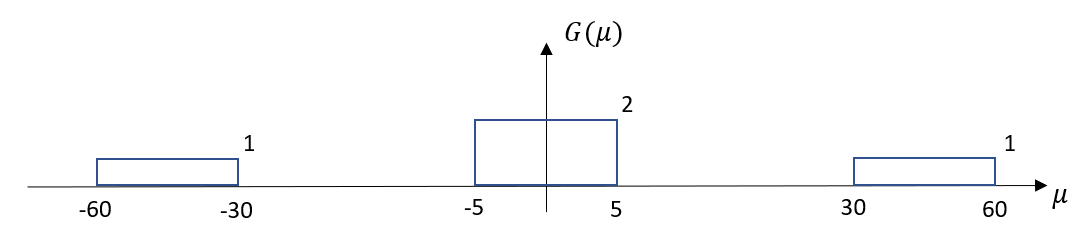
\includegraphics[width=\textwidth]{img/fig_6.png}
		\caption*{Rappresentazione grafica del segnale $G\left(\mu\right)$ nel dominio delle frequenze.}
	\end{figure}\newpage
	
	\subsection*{\textcolor{Green4}{\underline{\textbf{\emph{Passa basso ideale $\boldsymbol{a\left(t\right)}$}}}}}
	
	Il filtro passa basso ideale taglia le frequenze alte. Dato che per definizione è una box, la frequenza data rappresenta la metà della larghezza. Nel dominio del tempo viene rappresentato come una convoluzione, mentre nel dominio delle frequenze come una moltiplicazione. Quindi:
	\begin{equation*}
		\begin{array}{lll}
			\text{Dominio nel tempo} & \longrightarrow & a\left(t\right) = g\left(t\right) * 20\mathrm{sinc}\left(20t\right) \\
			\\
			\text{Dominio nelle frequenze} & \longrightarrow & A\left(\mu\right) = G\left(\mu\right) \cdot \Pi\left(\dfrac{\mu}{20}\right)
		\end{array}
	\end{equation*}
	\begin{figure}[!htp]
		\centering
		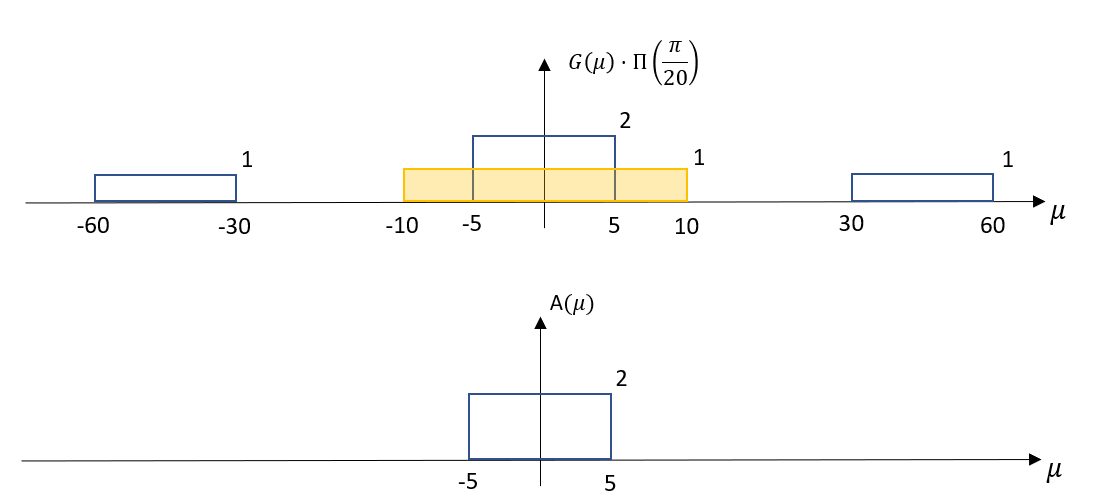
\includegraphics[width=\textwidth]{img/fig_7.png}
		\caption*{Rappresentazione grafica del segnale $A\left(\mu\right)$ nel dominio delle frequenze. Il grafico mostra la rappresentazione anche del filtro prima di applicarlo.}
	\end{figure}

	\subsection*{\textcolor{Green4}{\underline{\textbf{\emph{Campionatore $\boldsymbol{b\left(t\right)}$}}}}}
	
	Il campionamento non è altro che la moltiplicazione del segnale per un treno di impulsi. Quindi, la rappresentazione analitica del segnale è:
	\begin{equation*}
		\begin{array}{lllll}
			\text{Dominio nel tempo} & \longrightarrow & b\left(t\right) & = & a\left(t\right) \cdot \displaystyle\sum_{n} \delta\left(\dfrac{t - n}{10}\right) \\
			\\
			\text{Dominio nelle frequenze} & \longrightarrow & B\left(\mu\right) & = & A\left(\mu\right) * 10\displaystyle\sum_{n} \delta\left(\mu - 10n\right)\\
			\\
			&&& = & \int_{-\infty}^{\infty} A\left(\tau\right) \cdot 10\displaystyle\sum_{n} \delta\left(\mu -10n - \tau\right) \: \mathrm{d}\tau \\
			\\
			&&& \downarrow & \text{Porto fuori il } 10 \\
			\\
			&&& = & 10 \int_{-\infty}^{\infty} A\left(\tau\right) \cdot \displaystyle\sum_{n} \delta\left(\mu -10n - \tau\right) \: \mathrm{d}\tau \\
			\\
			&&& \downarrow & \text{Proprietà di setacciamento} \\
			\\
			&&& = & 10 \cdot \displaystyle\sum_{n} A\left(\mu - 10n\right)
		\end{array}
	\end{equation*}
	\begin{figure}[!htp]
		\centering
		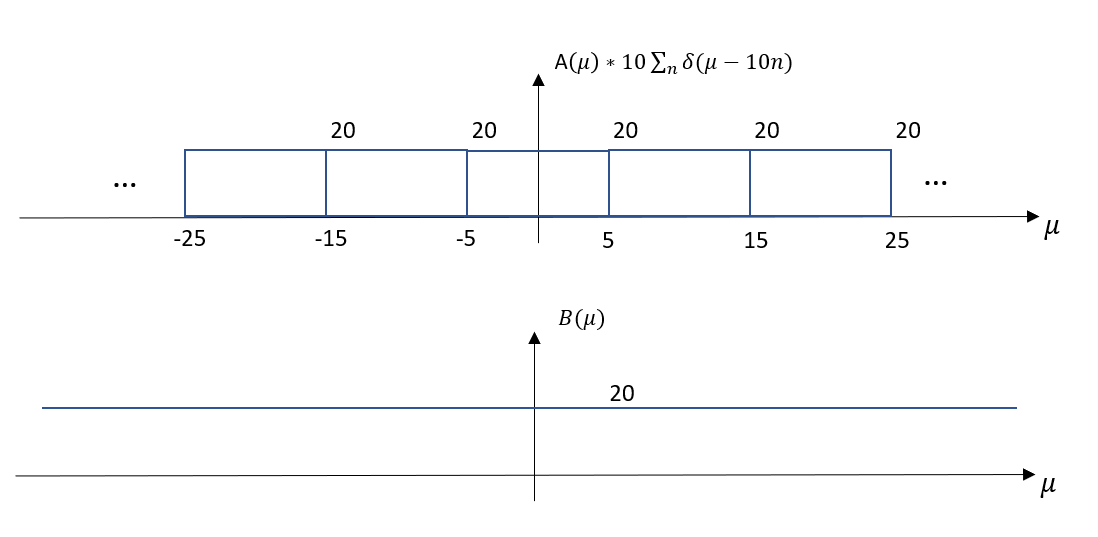
\includegraphics[width=\textwidth]{img/fig_8.png}
		\caption*{Rappresentazione grafica del segnale $B\left(\mu\right)$ nel dominio delle frequenze. Il grafico mostra la rappresentazione anche del campionamento dopo averlo applicato, ovvero non si manifesta aliasing ma appaiamento.}
	\end{figure}\newpage

	\subsection*{\textcolor{Green4}{\underline{\textbf{\emph{Passa basso ideale $\boldsymbol{c\left(t\right)}$}}}}}
	
	Ancora una volta, si applica un filtro passa basso ideale. A differenza di prima, adesso la frequenza di taglio (\emph{cutoff}) è pari a $25$ Hz, quindi la larghezza è pari a $50$:
	\begin{equation*}
		\begin{array}{lll}
			\text{Dominio nel tempo} & \longrightarrow & c\left(t\right) = b\left(t\right) * 50\mathrm{sinc}\left(50t\right) \\
			\\
			\text{Dominio nelle frequenze} & \longrightarrow & C\left(\mu\right) = B\left(\mu\right) \cdot \Pi\left(\dfrac{\mu}{50}\right)
		\end{array}
	\end{equation*}
	\begin{figure}[!htp]
		\centering
		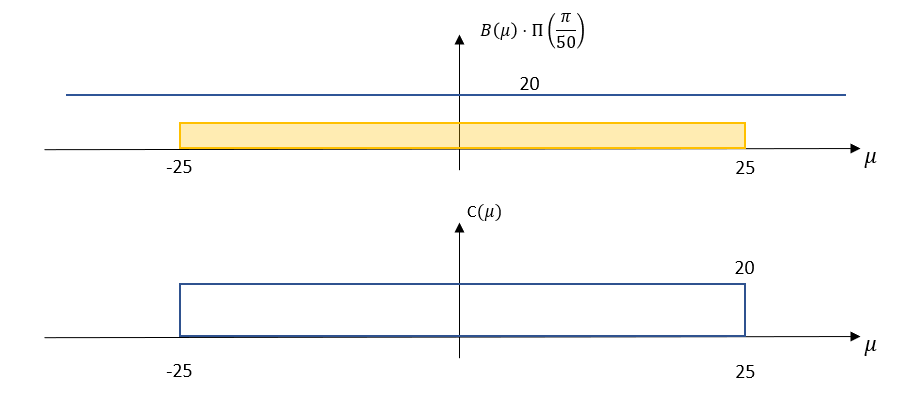
\includegraphics[width=\textwidth]{img/fig_9.png}
		\caption*{Rappresentazione grafica del segnale $C\left(\mu\right)$ nel dominio delle frequenze. Il grafico mostra la rappresentazione anche del filtro prima di applicarlo.}
	\end{figure}\newpage

	\section{Soluzione Esercizio}
	
	Prima di eseguire la convoluzione è necessario ottenere analiticamente i due segnali. Il segnale $x\left(t\right)$:
	\begin{equation*}
		\begin{array}{lll}
			\text{Dominio nelle frequenze} & \longrightarrow & X\left(\mu\right) = 2 \Pi\left(\dfrac{\mu - 1}{2}\right) \\
			\\
			\text{Dominio nel tempo} & \longrightarrow & x\left(t\right) = 4 \mathrm{sinc}\left(2t\right) \cdot e^{-j 2 \pi 1 t}
		\end{array}
	\end{equation*}
	Il segnale $h\left(t\right)$:
	\begin{equation*}
		\begin{array}{lll}
			\text{Dominio nelle frequenze} & \longrightarrow & H\left(\mu\right) = \delta\left(\mu-1\right) + \delta\left(\mu-2\right) \\
			\\
			\text{Dominio nel tempo} & \longrightarrow & h\left(t\right) = 1 \cdot e^{-j 2 \pi 1 t} + 1 \cdot e^{-j 2 \pi 2 t}
		\end{array}
	\end{equation*}
	Adesso è possibile eseguire la convoluzione. Per semplicità si esegue nel dominio delle frequenze, quindi:
	\begin{equation*}
		\begin{array}{lll}
			Y\left(\mu\right) & = & X\left(\mu\right) * H\left(\mu\right) \\
			\\
			& = & X\left(\mu\right) * \delta\left(\mu-1\right) + \delta\left(\mu-2\right) \\
			\\
			& = & \displaystyle\int_{-\infty}^{\infty} X\left(\tau\right) \cdot \left[\delta\left(\mu-1-\tau\right) + \delta\left(\mu-2-\tau\right)\right] \:\mathrm{d}\tau \\
			\\
			& = & \displaystyle\int_{-\infty}^{\infty} X\left(\tau\right) \cdot \delta\left(\mu - 1 -\tau\right) \:\mathrm{d}\tau + \displaystyle\int_{-\infty}^{\infty} X\left(\tau\right) \cdot \delta\left(\mu - 2 -\tau\right) \:\mathrm{d}\tau \\
			\\
			& \downarrow & \text{Proprietà di setacciamento} \\
			\\
			& = & X\left(\mu - 1\right) + X\left(\mu - 2\right) \\
			\\
			& = & 2\Pi\left(\dfrac{\mu - 1 - 1 }{2}\right) + 2\Pi\left(\dfrac{\mu - 1 - 2}{2}\right) \\
			\\
			& = & 2\Pi\left(\dfrac{\mu - 2}{2}\right) + 2\Pi\left(\dfrac{\mu - 3}{2}\right)
		\end{array}
	\end{equation*}\newpage
	
	\begin{figure}[!htp]
		\centering
		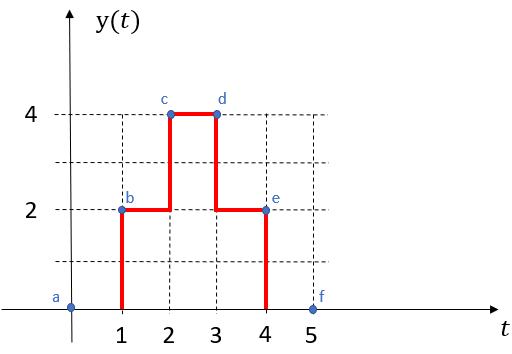
\includegraphics[width=.7\textwidth]{img/fig_10.png}
		\caption*{Rappresentazione grafica del segnale $Y\left(\mu\right)$ nel dominio delle frequenze dopo una convoluzione.}
	\end{figure}
	
	\noindent
	Tuttavia, l'esercizio richiede anche una descrizione grafica della convoluzione. Quindi, il grafico è il seguente:
	\begin{figure}[!htp]
		\centering
		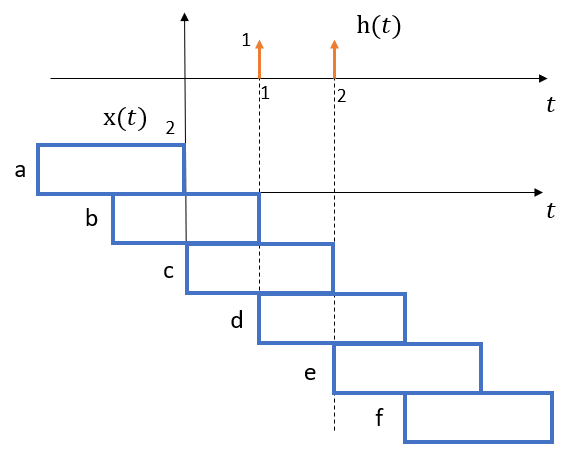
\includegraphics[width=.57\textwidth]{img/fig_11.png}
	\end{figure}
	\begin{enumerate}[label=\alph*)]
		\item Non vi è intersezione tra i segnali, quindi la risultante $y$ non esiste;
		
		\item Vi è intersezione con il primo impulso, il prodotto tra i segnali è un impulso di ampiezza $2$, quindi $y\left(1\right)=2$;
		
		\item Vi è una doppia intersezione con i due impulsi, il prodotto tra i segnali sono esattamente due impulsi di ampiezza (altezza) $2$ ciascuno, l'integrale del prodotto vale $4$, $y\left(2\right) = 4$;
		
		\item Vi è una doppia intersezione con i due impulsi, il prodotto tra i segnali sono esattamente due impulsi di ampiezza (altezza) $2$ ciascuno, l'integrale del prodotto vale $4$, $y\left(3\right) = 4$;
		
		\item Vi è intersezione con il secondo impulso, il prodotto tra i segnali è un impulso di ampiezza $2$, quindi $y\left(4\right)=2$;
		
		\item Non vi è intersezione tra i segnali, quindi la risultante $y$ non esiste.
	\end{enumerate}
	Adesso, si rappresenta graficamente il segnale $w\left(t\right)$:
	\begin{equation*}
		\begin{array}{lll}
			W\left(\mu\right) & = & \Pi\left(\dfrac{\mu - 1.5}{3}\right) - Y\left(\mu\right) \\
			\\
			& = & \Pi\left(\dfrac{\mu - 1.5}{3}\right) - 2\Pi\left(\dfrac{\mu - 2}{2}\right) + 2\Pi\left(\dfrac{\mu - 3}{2}\right)
		\end{array}
	\end{equation*}
	Il segno negativo ribalta il segnale $Y\left(\mu\right)$. Una volta ribaltato, si aumenta l'altezza applicando l'ampiezza del segnale $z\left(t\right)$:
	\begin{figure}[!htp]
		\centering
		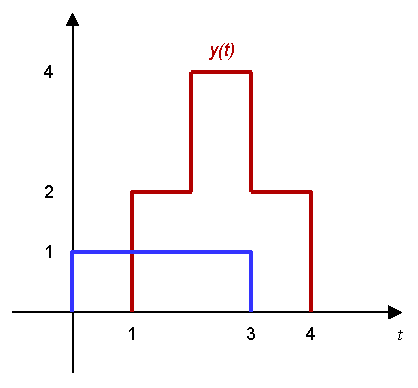
\includegraphics[width=.55\textwidth]{img/diff_1.pdf}
		\caption*{Rappresentazione grafica dei due segnali prima della differenza.}
	\end{figure}
	\begin{figure}[!htp]
		\centering
		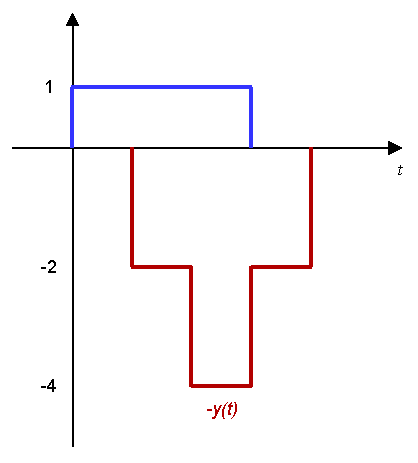
\includegraphics[width=.55\textwidth]{img/diff_2.pdf}
		\caption*{Rappresentazione grafica dopo il ribaltamento del segnale $Y\left(\mu\right)$.}
	\end{figure}\newpage

	\begin{figure}[!htp]
		\centering
		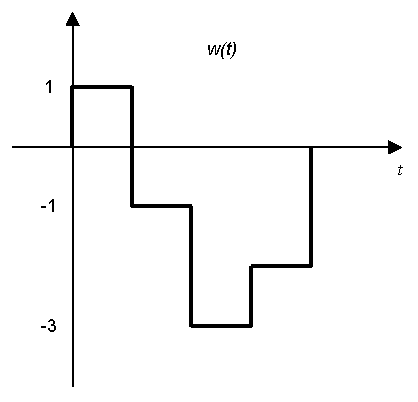
\includegraphics[width=.55\textwidth]{img/diff_3.pdf}
		\caption*{Rappresentazione grafica finale del segnale $W\left(\mu\right)$.}
	\end{figure}\newpage

	\section{Soluzione Esercizio}
	
	L'operazione di equalizzazione di un'immagine è un calcolo piuttosto semplice.\newline
	
	\noindent
	Il \textbf{primo passo} è numerare i livelli di grigio presenti all'interno dell'immagine. L'insieme dei livelli di grigio sarà denotato con la lettera $r_{k}$ e con la lettera $k$ si indicherà il $k$-esimo livello di grigio. Quindi, si riporta per comodità la matrice e si elencano i livelli di grigio:
	\begin{table}[!htbp]
		\centering
		\begin{tabular}{@{} c | c | c | c @{}}
			\toprule
			0 & 0 & 1 & 3 \\
			1 & 0 & 4 & 5 \\
			7 & 2 & 0 & 6 \\
			7 & 4 & 7 & 7 \\
			\bottomrule
		\end{tabular}
	\end{table}
	\begin{equation*}
		r_{k} = \left\{0, 1, 2, 3, 4, 5, 6, 7\right\} \hspace{2em} \text{con } r_{1} = 0, r_{2} = 1, ..., r_{8} = 7
	\end{equation*}
	In altre parole, l'insieme indica tutti i possibili valori che ci sono all'interno della matrice in ordine crescente.\newline
	
	\noindent
	Il \textbf{secondo passo} è contare le occorrenze di ogni elemento di $r_{k}$. L'insieme delle occorrenze sarà indicato con $H\left(r_{k}\right)$:
	\begin{equation*}
		\begin{array}{rlllllllll}
			r_{k} 				& = & 0,& 1,& 2,& 3,& 4,& 5,& 6,& 7 \\
			\\
			H\left(r_{k}\right) & = & 4,& 2,& 1,& 1,& 2,& 1,& 1,& 4
		\end{array}
	\end{equation*}
	Quindi, lo zero si ripete $4$ volte all'interno della matrice, l'uno si ripete $2$ volte, il due si ripete una volta e così via fino al valore $7$ che si ripete $4$ volte.\newline
	
	\noindent
	Il \textbf{terzo passo} è applicare la seguente formula, che rappresenta una sorta di probabilità:
	\begin{equation*}
		p_{r}\left(r_{k}\right) = \dfrac{H\left(r_{k}\right)}{M \cdot N}
	\end{equation*}
	In cui $M,N$ sono il numero di righe e colonne della matrice, quindi $4 \times 4 = 16$. Si applica a ciascun elemento dell'insieme $r_{k}$:
	\begin{equation*}
		\begin{array}{rccccccccc}
			r_{k} 					& = & 0,& 1,& 2,& 3,& 4,& 5,& 6,& 7 \\
			\\
			H\left(r_{k}\right) 	& = & 4,& 2,& 1,& 1,& 2,& 1,& 1,& 4 \\
			\\
			p_{r}\left(r_{k}\right) & = & \dfrac{4}{16},& \dfrac{2}{16},& \dfrac{1}{16},& \dfrac{1}{16},& \dfrac{2}{16},& \dfrac{1}{16},& \dfrac{1}{16},& \dfrac{4}{16}
		\end{array}
	\end{equation*}\newpage

	\noindent
	Il \textbf{quarto passo} è la normalizzazione, indicata con $S$ dei valori. Essa è una somma cumulativa dei valori $p_{r}\left(r_{k}\right)$ e ciascun valore, della somma, si moltiplica per il valore massimo di grigio (in questo caso $7$):
	\begin{equation*}
		\begin{array}{rccccccccc}
			r_{k} 						& = & 0,& 1,& 2,& 3,& 4,& 5,& 6,& 7 \\
			\\
			H\left(r_{k}\right) 		& = & 4,& 2,& 1,& 1,& 2,& 1,& 1,& 4 \\
			\\
			p_{r}\left(r_{k}\right) 	& = & \dfrac{4}{16},& \dfrac{2}{16},& \dfrac{1}{16},& \dfrac{1}{16},& \dfrac{2}{16},& \dfrac{1}{16},& \dfrac{1}{16},& \dfrac{4}{16} \\
			\\
			\sum p_{r}\left(r_{k}\right)& = & \dfrac{4}{16},& \dfrac{6}{16},& \dfrac{7}{16},& \dfrac{8}{16},& \dfrac{10}{16},& \dfrac{11}{16},& \dfrac{12}{16},& \dfrac{16}{16}
		\end{array}
	\end{equation*}
	Adesso che è stata esplicitata la somma cumulativa, si moltiplica ogni frazione per il valore massimo di grigio ($7$) e poi si esegue un arrotondamento per eccesso da $0.5$ a $0.9$, altrimenti per difetto:
	\begin{equation*}
		\begin{array}{lllllll}
			r_{k} = 0 & \longrightarrow & \dfrac{4}{16} \cdot 7 & = & 1.75 & \longrightarrow & 2 \\
			\\
			r_{k} = 1 & \longrightarrow & \dfrac{6}{16} \cdot 7 & = & 2.625 & \longrightarrow & 3 \\
			\\
			r_{k} = 2 & \longrightarrow & \dfrac{7}{16} \cdot 7 & = & 3.0625 & \longrightarrow & 3 \\
			\\
			r_{k} = 3 & \longrightarrow & \dfrac{8}{16} \cdot 7 & = & 3.5 & \longrightarrow & 4 \\
			\\
			r_{k} = 4 & \longrightarrow & \dfrac{10}{16} \cdot 7 & = & 4.375 & \longrightarrow & 4 \\
			\\
			r_{k} = 5 & \longrightarrow & \dfrac{11}{16} \cdot 7 & = & 4.8125 & \longrightarrow & 5 \\
			\\
			r_{k} = 6 & \longrightarrow & \dfrac{12}{16} \cdot 7 & = & 5.25 & \longrightarrow & 5 \\
			\\
			r_{k} = 7 & \longrightarrow & \dfrac{16}{16} \cdot 7 & = & 7 & \longrightarrow & 7
		\end{array}
	\end{equation*}\newline

	\noindent
	Il \textbf{quinto e ultimo passo} è riscrivere la matrice equalizzata andando a sostituire i valori $r_{k}$ con la rispettiva normalizzazione (quindo gli zero con $2$, gli uni con $3$, e così via):
	\begin{table}[!htbp]
		\centering
		\begin{tabular}{@{} c | c | c | c @{}}
			\toprule
			2 & 2 & 3 & 4 \\
			3 & 2 & 4 & 5 \\
			7 & 3 & 2 & 5 \\
			7 & 4 & 7 & 7 \\
			\bottomrule
		\end{tabular}
	\end{table}
\end{document}